%% bare_conf.tex
%% V1.4b
%% 2015/08/26
%% by Michael Shell
%% See:
%% http://www.michaelshell.org/
%% for current contact information.
%%
%% This is a skeleton file demonstrating the use of IEEEtran.cls
%% (requires IEEEtran.cls version 1.8b or later) with an IEEE
%% conference paper.
%%
%% Support sites:
%% http://www.michaelshell.org/tex/ieeetran/
%% http://www.ctan.org/pkg/ieeetran
%% and
%% http://www.ieee.org/

%%*************************************************************************
%% Legal Notice:
%% This code is offered as-is without any warranty either expressed or
%% implied; without even the implied warranty of MERCHANTABILITY or
%% FITNESS FOR A PARTICULAR PURPOSE! 
%% User assumes all risk.
%% In no event shall the IEEE or any contributor to this code be liable for
%% any damages or losses, including, but not limited to, incidental,
%% consequential, or any other damages, resulting from the use or misuse
%% of any information contained here.
%%
%% All comments are the opinions of their respective authors and are not
%% necessarily endorsed by the IEEE.
%%
%% This work is distributed under the LaTeX Project Public License (LPPL)
%% ( http://www.latex-project.org/ ) version 1.3, and may be freely used,
%% distributed and modified. A copy of the LPPL, version 1.3, is included
%% in the base LaTeX documentation of all distributions of LaTeX released
%% 2003/12/01 or later.
%% Retain all contribution notices and credits.
%% ** Modified files should be clearly indicated as such, including  **
%% ** renaming them and changing author support contact information. **
%%*************************************************************************


% *** Authors should verify (and, if needed, correct) their LaTeX system  ***
% *** with the testflow diagnostic prior to trusting their LaTeX platform ***
% *** with production work. The IEEE's font choices and paper sizes can   ***
% *** trigger bugs that do not appear when using other class files.       ***                          ***
% The testflow support page is at:
% http://www.michaelshell.org/tex/testflow/



\documentclass[conference]{IEEEtran}
% Some Computer Society conferences also require the compsoc mode option,
% but others use the standard conference format.
%
% If IEEEtran.cls has not been installed into the LaTeX system files,
% manually specify the path to it like:
% \documentclass[conference]{../sty/IEEEtran}





% Some very useful LaTeX packages include:
% (uncomment the ones you want to load)


% *** MISC UTILITY PACKAGES ***
%
%\usepackage{ifpdf}
% Heiko Oberdiek's ifpdf.sty is very useful if you need conditional
% compilation based on whether the output is pdf or dvi.
% usage:
% \ifpdf
%   % pdf code
% \else
%   % dvi code
% \fi
% The latest version of ifpdf.sty can be obtained from:
% http://www.ctan.org/pkg/ifpdf
% Also, note that IEEEtran.cls V1.7 and later provides a builtin
% \ifCLASSINFOpdf conditional that works the same way.
% When switching from latex to pdflatex and vice-versa, the compiler may
% have to be run twice to clear warning/error messages.






% *** CITATION PACKAGES ***
%
\usepackage{cite}
% cite.sty was written by Donald Arseneau
% V1.6 and later of IEEEtran pre-defines the format of the cite.sty package
% \cite{} output to follow that of the IEEE. Loading the cite package will
% result in citation numbers being automatically sorted and properly
% "compressed/ranged". e.g., [1], [9], [2], [7], [5], [6] without using
% cite.sty will become [1], [2], [5]--[7], [9] using cite.sty. cite.sty's
% \cite will automatically add leading space, if needed. Use cite.sty's
% noadjust option (cite.sty V3.8 and later) if you want to turn this off
% such as if a citation ever needs to be enclosed in parenthesis.
% cite.sty is already installed on most LaTeX systems. Be sure and use
% version 5.0 (2009-03-20) and later if using hyperref.sty.
% The latest version can be obtained at:
% http://www.ctan.org/pkg/cite
% The documentation is contained in the cite.sty file itself.





% *** GRAPHICS RELATED PACKAGES ***
%
\ifCLASSINFOpdf
	 \usepackage[pdftex]{graphicx}
	 %declare the path(s) where your graphic files are
	 \graphicspath{{figure/}}
	 %and their extensions so you won't have to specify these with
	 %every instance of \includegraphics
	 \DeclareGraphicsExtensions{.pdf,.jpeg,.png}
\else
  % or other class option (dvipsone, dvipdf, if not using dvips). graphicx
  % will default to the driver specified in the system graphics.cfg if no
  % driver is specified.
  % \usepackage[dvips]{graphicx}
  % declare the path(s) where your graphic files are
  % \graphicspath{{../eps/}}
  % and their extensions so you won't have to specify these with
  % every instance of \includegraphics
  % \DeclareGraphicsExtensions{.eps}
\fi
% graphicx was written by David Carlisle and Sebastian Rahtz. It is
% required if you want graphics, photos, etc. graphicx.sty is already
% installed on most LaTeX systems. The latest version and documentation
% can be obtained at: 
% http://www.ctan.org/pkg/graphicx
% Another good source of documentation is "Using Imported Graphics in
% LaTeX2e" by Keith Reckdahl which can be found at:
% http://www.ctan.org/pkg/epslatex
%
% latex, and pdflatex in dvi mode, support graphics in encapsulated
% postscript (.eps) format. pdflatex in pdf mode supports graphics
% in .pdf, .jpeg, .png and .mps (metapost) formats. Users should ensure
% that all non-photo figures use a vector format (.eps, .pdf, .mps) and
% not a bitmapped formats (.jpeg, .png). The IEEE frowns on bitmapped formats
% which can result in "jaggedy"/blurry rendering of lines and letters as
% well as large increases in file sizes.
%
% You can find documentation about the pdfTeX application at:
% http://www.tug.org/applications/pdftex





% *** MATH PACKAGES ***
%
\usepackage{amsmath}
% A popular package from the American Mathematical Society that provides
% many useful and powerful commands for dealing with mathematics.
%
% Note that the amsmath package sets \interdisplaylinepenalty to 10000
% thus preventing page breaks from occurring within multiline equations. Use:
%\interdisplaylinepenalty=2500
% after loading amsmath to restore such page breaks as IEEEtran.cls normally
% does. amsmath.sty is already installed on most LaTeX systems. The latest
% version and documentation can be obtained at:
% http://www.ctan.org/pkg/amsmath





% *** SPECIALIZED LIST PACKAGES ***
%
%\usepackage{algorithmic}
% algorithmic.sty was written by Peter Williams and Rogerio Brito.
% This package provides an algorithmic environment fo describing algorithms.
% You can use the algorithmic environment in-text or within a figure
% environment to provide for a floating algorithm. Do NOT use the algorithm
% floating environment provided by algorithm.sty (by the same authors) or
% algorithm2e.sty (by Christophe Fiorio) as the IEEE does not use dedicated
% algorithm float types and packages that provide these will not provide
% correct IEEE style captions. The latest version and documentation of
% algorithmic.sty can be obtained at:
% http://www.ctan.org/pkg/algorithms
% Also of interest may be the (relatively newer and more customizable)
% algorithmicx.sty package by Szasz Janos:
% http://www.ctan.org/pkg/algorithmicx




% *** ALIGNMENT PACKAGES ***
%
\usepackage{array}
% Frank Mittelbach's and David Carlisle's array.sty patches and improves
% the standard LaTeX2e array and tabular environments to provide better
% appearance and additional user controls. As the default LaTeX2e table
% generation code is lacking to the point of almost being broken with
% respect to the quality of the end results, all users are strongly
% advised to use an enhanced (at the very least that provided by array.sty)
% set of table tools. array.sty is already installed on most systems. The
% latest version and documentation can be obtained at:
% http://www.ctan.org/pkg/array


% IEEEtran contains the IEEEeqnarray family of commands that can be used to
% generate multiline equations as well as matrices, tables, etc., of high
% quality.




% *** SUBFIGURE PACKAGES ***
%\ifCLASSOPTIONcompsoc
%  \usepackage[caption=false,font=normalsize,labelfont=sf,textfont=sf]{subfig}
%\else
%  \usepackage[caption=false,font=footnotesize]{subfig}
%\fi
% subfig.sty, written by Steven Douglas Cochran, is the modern replacement
% for subfigure.sty, the latter of which is no longer maintained and is
% incompatible with some LaTeX packages including fixltx2e. However,
% subfig.sty requires and automatically loads Axel Sommerfeldt's caption.sty
% which will override IEEEtran.cls' handling of captions and this will result
% in non-IEEE style figure/table captions. To prevent this problem, be sure
% and invoke subfig.sty's "caption=false" package option (available since
% subfig.sty version 1.3, 2005/06/28) as this is will preserve IEEEtran.cls
% handling of captions.
% Note that the Computer Society format requires a larger sans serif font
% than the serif footnote size font used in traditional IEEE formatting
% and thus the need to invoke different subfig.sty package options depending
% on whether compsoc mode has been enabled.
%
% The latest version and documentation of subfig.sty can be obtained at:
% http://www.ctan.org/pkg/subfig




% *** FLOAT PACKAGES ***
%
%\usepackage{fixltx2e}
% fixltx2e, the successor to the earlier fix2col.sty, was written by
% Frank Mittelbach and David Carlisle. This package corrects a few problems
% in the LaTeX2e kernel, the most notable of which is that in current
% LaTeX2e releases, the ordering of single and double column floats is not
% guaranteed to be preserved. Thus, an unpatched LaTeX2e can allow a
% single column figure to be placed prior to an earlier double column
% figure.
% Be aware that LaTeX2e kernels dated 2015 and later have fixltx2e.sty's
% corrections already built into the system in which case a warning will
% be issued if an attempt is made to load fixltx2e.sty as it is no longer
% needed.
% The latest version and documentation can be found at:
% http://www.ctan.org/pkg/fixltx2e


%\usepackage{stfloats}
% stfloats.sty was written by Sigitas Tolusis. This package gives LaTeX2e
% the ability to do double column floats at the bottom of the page as well
% as the top. (e.g., "\begin{figure*}[!b]" is not normally possible in
% LaTeX2e). It also provides a command:
%\fnbelowfloat
% to enable the placement of footnotes below bottom floats (the standard
% LaTeX2e kernel puts them above bottom floats). This is an invasive package
% which rewrites many portions of the LaTeX2e float routines. It may not work
% with other packages that modify the LaTeX2e float routines. The latest
% version and documentation can be obtained at:
% http://www.ctan.org/pkg/stfloats
% Do not use the stfloats baselinefloat ability as the IEEE does not allow
% \baselineskip to stretch. Authors submitting work to the IEEE should note
% that the IEEE rarely uses double column equations and that authors should try
% to avoid such use. Do not be tempted to use the cuted.sty or midfloat.sty
% packages (also by Sigitas Tolusis) as the IEEE does not format its papers in
% such ways.
% Do not attempt to use stfloats with fixltx2e as they are incompatible.
% Instead, use Morten Hogholm'a dblfloatfix which combines the features
% of both fixltx2e and stfloats:
%
% \usepackage{dblfloatfix}
% The latest version can be found at:
% http://www.ctan.org/pkg/dblfloatfix




% *** PDF, URL AND HYPERLINK PACKAGES ***
%
\usepackage{url}
% url.sty was written by Donald Arseneau. It provides better support for
% handling and breaking URLs. url.sty is already installed on most LaTeX
% systems. The latest version and documentation can be obtained at:
% http://www.ctan.org/pkg/url
% Basically, \url{my_url_here}.



% *** Do not adjust lengths that control margins, column widths, etc. ***
% *** Do not use packages that alter fonts (such as pslatex).         ***
% There should be no need to do such things with IEEEtran.cls V1.6 and later.
% (Unless specifically asked to do so by the journal or conference you plan
% to submit to, of course. )

\usepackage{float}

% correct bad hyphenation here
\hyphenation{op-tical net-works semi-conduc-tor}

\begin{document}
%
% paper title
% Titles are generally capitalized except for words such as a, an, and, as,
% at, but, by, for, in, nor, of, on, or, the, to and up, which are usually
% not capitalized unless they are the first or last word of the title.
% Linebreaks \\ can be used within to get better formatting as desired.
% Do not put math or special symbols in the title.
\title{Unstructured Document Recognition \\on Business Invoice}


% author names and affiliations
% use a multiple column layout for up to three different
% affiliations
\author{\IEEEauthorblockN{Wenshun Liu, Billy Wan, Yaqi Zhang}
\IEEEauthorblockA{
Email: wl88@stanford.edu, xwan@stanford.edu, yaqiz@stanford.edu}
}

%\author{\IEEEauthorblockN{Yaqi Zhang}
%\IEEEauthorblockA{Department of Electrical Engineering\\
%Stanford University\\
%Stanford, California 94305\\
%Email: yaqiz@stanford.edu}
%}

% use for special paper notices
\IEEEspecialpapernotice{
	\large CS229: Machine Learning 
}

% make the title area
\maketitle

% As a general rule, do not put math, special symbols or citations
% in the abstract
\begin{abstract}

This project describes a bag-of-words approach for business invoice recognition. Bags of potential features are generated to capture layout and textual properties for each field of interest, and weighted to reveal key factors that identify a field. Feature selection, threshold tuning, and model comparison are evaluated. Overall, we achieved 8.81\% for training error and 13.99\% for testing error. 

\end{abstract}


\IEEEpeerreviewmaketitle

\section{Introduction}
Invoice processing is one of the most critical tasks for the financial department of any organization. In many of such departments, invoices are still examined and entered manually, a process that is slow, costly, prone to human errors, and has become a bottleneck of high-speed data processes especially when the number of invoices grows dramatically with the development of the social economy \cite{ming2003research}. While a standard list of critical fields is usually visible in almost all invoices, the choice of keywords and layout can vary largely from vendor to vendor, creating the challenge of extracting structured information from unstructured documents in an attempt to automate such invoice recognition and entry process.

The invoice recognition model this project proposes intends to yield additional insights to this problem. 8 fields of interests (including a negative class) are identified and recognized under the process outlined in Fig. \ref{fig:flow1}. 

The raw inputs are scanned invoice images. After image processing, OCR, and pattern matching steps, a list of word groups (tokens) and coordinates are extracted from the original images, and are used as the actual input for the model. Bags of potential features are generated from the actual inputs under a set of feature selection rules to capture various layout properties and word patterns for each field, and then weighted using 3 classification models (Naive Bayes, Logistic Regression, and SVM) to output a predicted field for every word group.

\begin{figure}
\centering
\begin{minipage}{.5\linewidth}
  \centering
  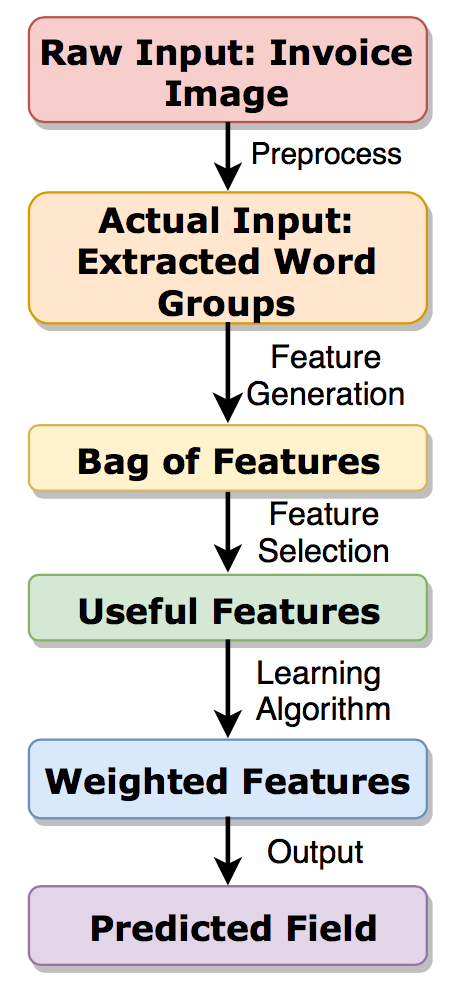
\includegraphics[width=.5\linewidth]{flow_1}
  \caption{Flow of Invoice Recognition}
  \label{fig:flow1}
\end{minipage}%
\begin{minipage}{.5\linewidth}
  \centering
  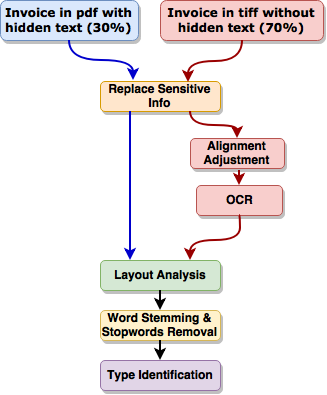
\includegraphics[width=.9\linewidth]{flow}
  \caption{Flow of Data Preprocessing}
  \label{fig:flow2}
\end{minipage}
\end{figure}


\section{Related Work}
Numerous image processing and machine learning attempts have been made to tackle the invoice recognition problem from different angles. 

Image processing approaches rely on column detection and word sequence recognition within each logically segmented region \cite{marinai2008introduction}, with the occasional aid of machine learning techniques for more precise region classification results. While image processing techniques \cite{zhou2000hough} can be of great aid to many other models, a recognition algorithm centered around it overly simplifies the complex nature of invoice layout, and assumes homogeneous properties in region segmentation based on linear combination of rules, which is almost never the case in practice given the unpredictable nature of invoice layout.

In need of more complex models leveraging machine learning techniques, template based classification algorithms are proposed, where the template of an invoice (calculated and represented by a set of layout attributes) is either matched against a template library \cite{ming2003research}\cite{sorio2013machine}, or is assigned to a cluster of templates sharing similar properties \cite{hamza2008incremental}. In either approach, the template library or cluster constantly expands when no obvious match exists.

Template based models have the obvious benefit of being able to recognize the entire invoice all at once through pre-established template-specific rules, and perform the best with high quality images and highly distinctive templates. Unfortunately, neither is guaranteed in reality as invoices are often poorly scanned, and the huge vendor (and thus invoice template) pool implies frequent occurrence of invoices with similar structure but minor (yet crucial) variance in layout and field arrangements. In the case of template library, this could cause critical fields to be mis-recognized following incorrect rules. In the case of clusters, defining template "distance" and distinguishing minor variance within a cluster are themselves tricky and error-prone. Such models are also memory-intensive as the library or cluster size constantly expands.

Also available are rule-based models, where sets of hand-crafted rules are weighted to capture micro-level details for each field \cite{belaid2004morphological}. Such approaches avoid the inflexibility when an invoice is treated as a whole. While hand-crafted rules work well with invoices containing industry standard components and layout, they imply presumptions on field properties that are either incorrectly arbitrary (e.g., amounts are not always right aligned) or simply not achievable (e.g., match price and quantity with amount to identify invoice lines while not all three fields are present in many real-world invoices).

The model proposed in this project also performs field-by-field recognition, though instead of merely determining the weights of hand-crafted rules, a bag of potential features is supplied to generate the best set of rules that should be used.


\section{Dataset and Features}
\subsection{Dataset Generation}
\label{sec:dandf}
\begin{figure}[H]
\centering
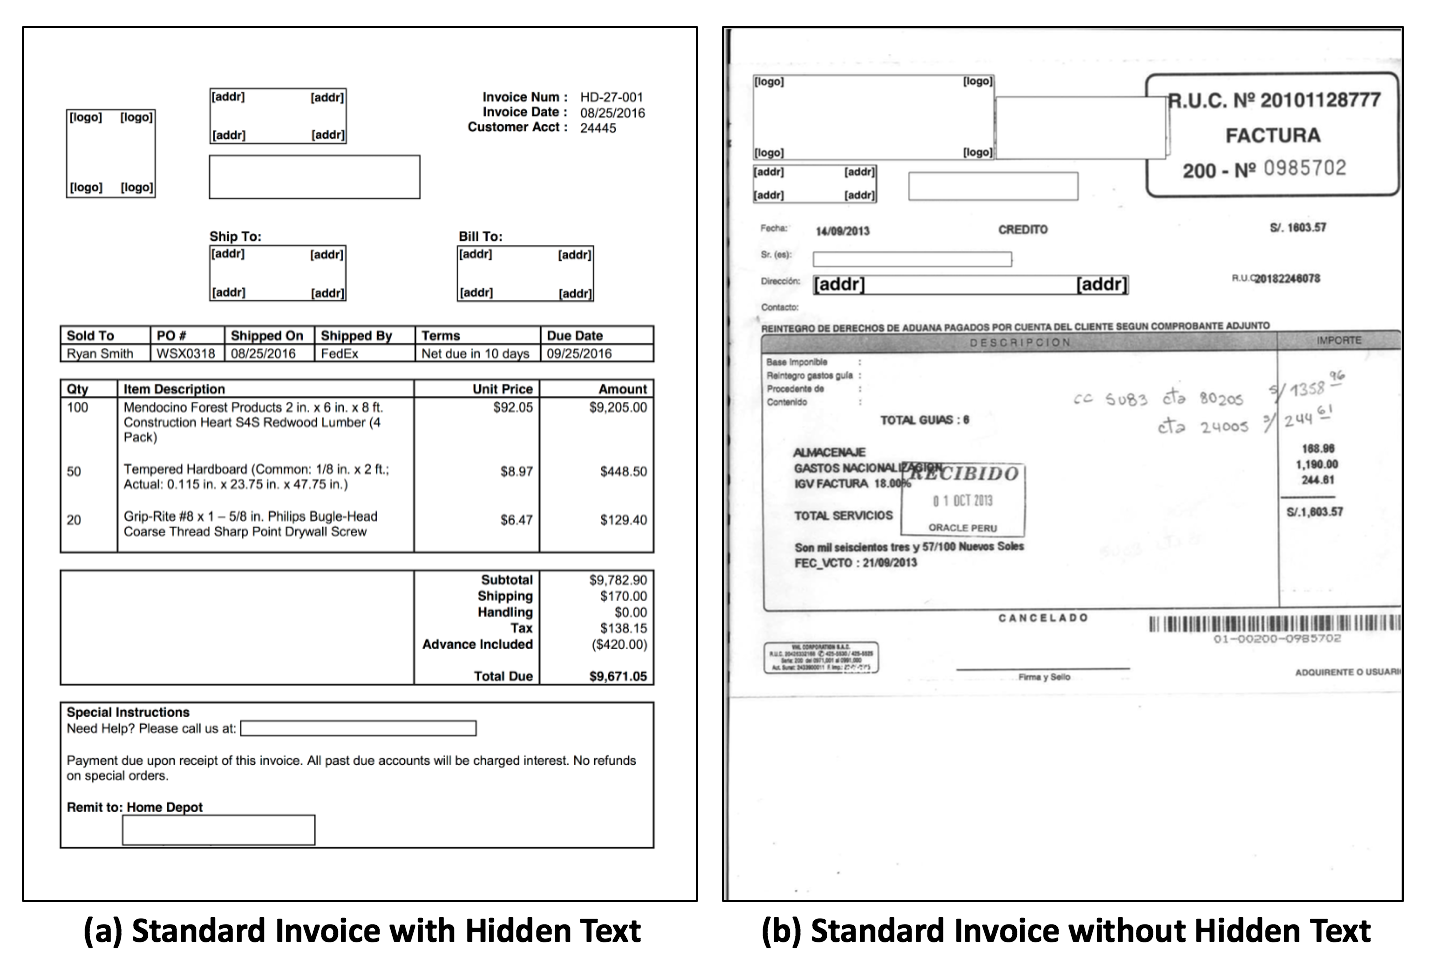
\includegraphics[width=1\linewidth]{invoiceexp.png}
\caption{Sample Invoices}
\label{fig:invoiceexp}
\end{figure}
% \begin{figure}[H]
% \centering
% 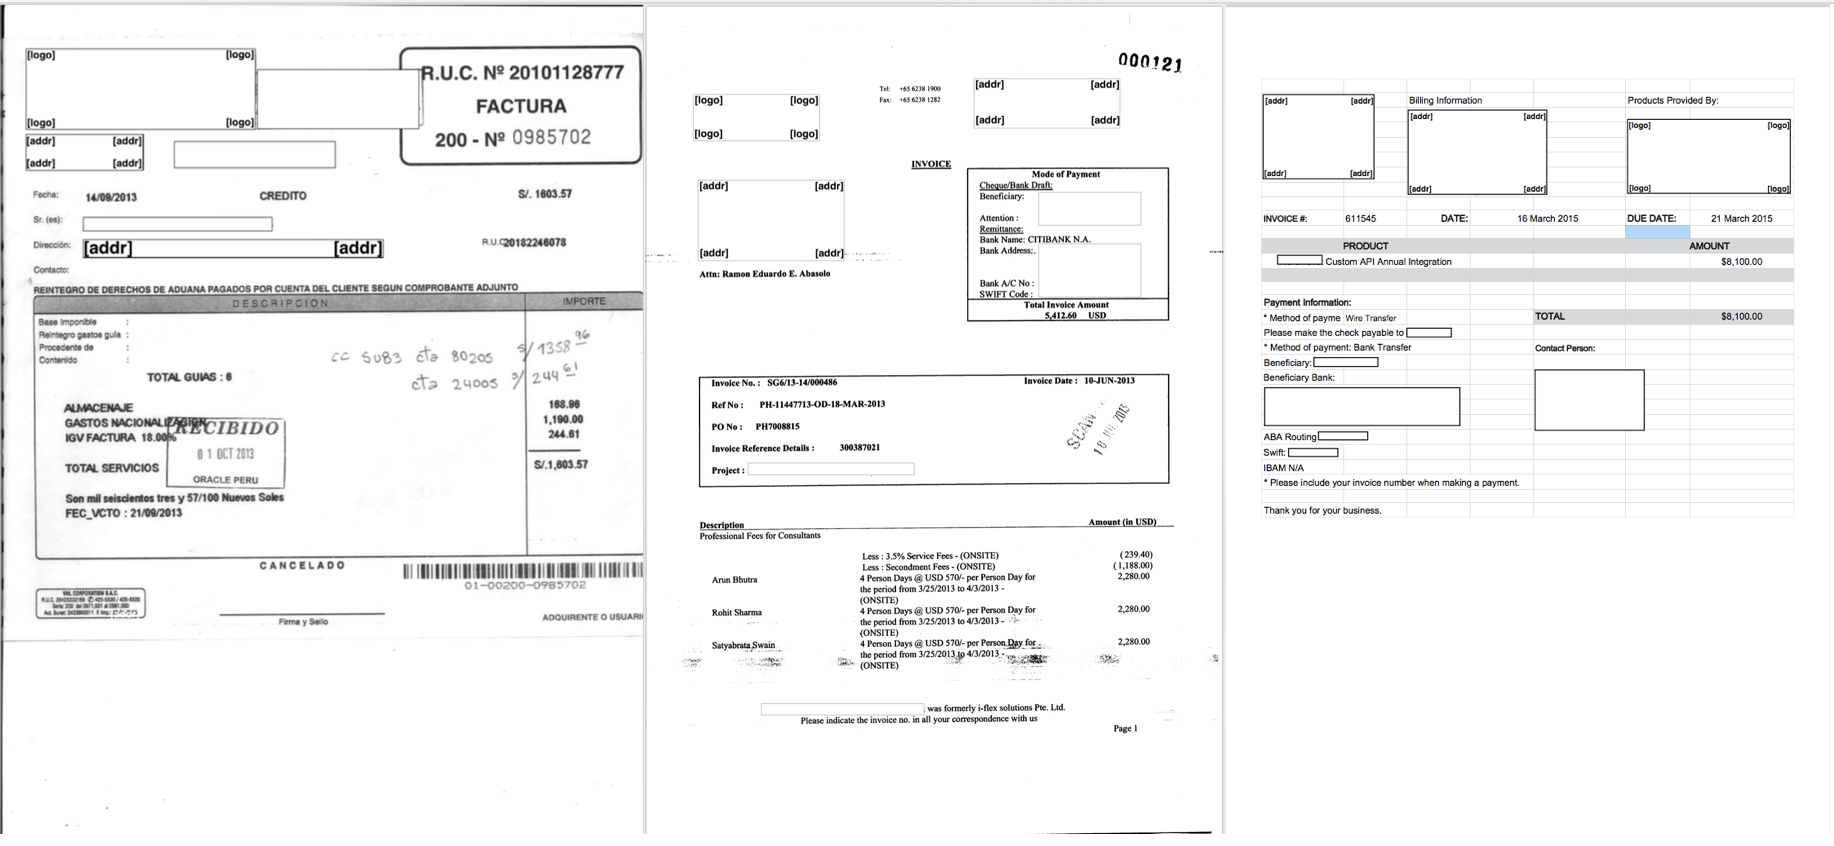
\includegraphics[width=1\linewidth]{nonstandardinvoice.png}
% \caption{Sample Non-standard Invoice without hidden text}
% \label{fig:nonstandardinvoice}
% \end{figure}

97 raw invoice images are obtained from the internal testing library of Oracle Corporation, examples of which are displayed in Fig. \ref{fig:invoiceexp}. Sensitive information has been manually replaced with tokens (LOGO, ADDR, etc) labeled on the corners of the bounding boxes, to preserve position without revealing the actual text. While some are well-formatted PDF files with hidden text, most are TIFF images that require additional steps before PDF Layout Analysis\cite{shinyamapdfminer} can take place to extract word groups. The process of generating word groups and coordinates as actual training input is outlined  in Fig. \ref{fig:flow2}

TIFF images are first rotated to best alignment with rotation angle calculated from Hough Line Transform\cite{vc1962method}, and then performed Optical Character Recognition (OCR)\cite{smith2007overview} to obtain any textual groups exist in the image. All sample invoices are then sent to PDF Layout Analysis, where coordinates of tokenized textual groups are retrieved and stored. Then, additional word processing is implemented on each token, including Porter2 word stemming\cite{stemming}, stopwords removal\cite{loper205028nltk}, and type identification using regular expressions. 5 special types - DATE, MONEY, NUMBER, TELE, and EMAIL - are defined for the last process, where the exact textual values are substituted for more generic representation.

\subsection{Feature Generation}
For each token, the following set of feature selection rules is applied: horizontally aligned tokens, vertically aligned tokens, nearby tokens within a distance threshold, overall vertical position, and its own type. The resulting features from each token are then accumulated to form the bag of potential features, where binary values are used to track whether any given feature exists for a token. For instance, if token $A$ is horizontally aligned with token $B$, feature $B\_halign$ will be generated and be of value $1$ for $A$ and 0 otherwise. The feature selection rules are picked to capture basic layout information, without presumption of any standard template.

Around 8000 features were generated for the 2095 tokens ($m=2095$) in 97 invoices, and further reduced through preliminary feature pruning
(Section~\ref{sec:dandf}) to exclude the ones that only appear once (and are thus not indicative). The remaining features ($n\approx2000$) are then put into careful feature selection process detailed in Section $V$.

\section{Methods}
Using the scikit-learn library\cite{scikit-learn}, three learning models were trained and used to make predictions: Multinomial Naive Bayes, Logistic Regression, and Support Vector Machines (SVM). In all three models, the class labels $y\in[0, 7]$, where 0 is the negative class, and 1-7 corresponds to \textit{invoice number}, \textit{invoice date}, \textit{total amount}, \textit{PO \#}, \textit{payment terms}, \textit{due date}, and \textit{tax}, respectively.
\subsection{Multinomial Naive Bayes}
In the Multinomial Naive Bayes model, we make the assumption that the features $x_i$ are conditionally independent given the class labels y. We used this model with Laplace smoothing to fit parameters $\phi_{y=k}=p(y=k)$, and $\phi_{j, y=k} = p(x_j=1\vert y=k)$, where $k\in[0,7]$, in order to maximize the joint likelihood of the data, given by
\begin{align*}
\mathcal{L}(\phi_{y=k}, \phi_{j, y=k}) = \prod_{i=1}^mp(x^{(i)}, y^{(i)}).
\end{align*}
The maximum likelihood estimation of these parameters are given as follows:
\begin{align*}
\phi_{y=k} &= \frac{\sum_{i=1}^m{\bf 1}(y^{(i)}=k)}{m}\\
\phi_{j, y=k} &= \frac{\sum_{i=1}^m{\bf 1}(x_j^{(i)}=1, y^{(i)}=k)+1}{m+K}.
\end{align*}
After fitting these parameters, to make a prediction on a new example with feature $x$, we calculate the posterior probability for each class $k$ using
\begin{align*}
p(y=k\vert x) &= \frac{p(x\vert y=k)p(y=k)}{p(x)} \\
&= \frac{(\prod_{i=1}^np(x_i\vert y=k))p(y=k)}{\sum_{l=1}^K(\prod_{i=1}^np(x_i\vert y=l))p(y=l)}
\end{align*}
and substituting the probabilities with the corresponding parameters. The class with the highest posterior probability will then be our prediction.

\subsection{Logistic Regression}
In the Logistic Regression model, we first transform our multiclass classification problem into a binary classification problem using the one-vs-rest approach, i.e.\ when calculating the probability for class $k$, all other classes have the same label. In binary Logistic Regression, we use the following hypothesis to make predictions:
\begin{align*}
h_{\theta}(x) = \frac{1}{1+\exp(-\theta^Tx)}.
\end{align*}
This hypothesis indicates that a logistic/sigmoid curve, which smoothly increases from 0 to 1, is fit to the data such that we predict 1 when $h_\theta(x) > 0.5$ and 0 otherwise. Then, we choose the logistic loss
\begin{align*}
\mathrm{L}(z, y) &= \log(1+\exp(-yz))\\
&= \log(1+\exp(-y\theta^Tx)),
\end{align*}
where $z=\theta^Tx$. The loss is minimized when we have a large margin $yz$, and maximized otherwise. $\ell_2$-regularization is used to combat overfitting. We used a slight variation of empirical regularized risk function than the one from class note to minimize:
\begin{align}\label{eq:logreg}
J_C(\theta) &= \frac{C}{m}\sum_{i=1}^m\mathrm{L}(\theta^Tx^{(i)}, y^{(i)}) + \frac{1}{2}\lVert\theta\rVert_2^2\\
&= \frac{C}{m}\sum_{i=1}^m\log(1+\exp(-y^{(i)}\theta^Tx^{(i)})) + \frac{1}{2}\lVert\theta\rVert_2^2.
\end{align}
The scikit-learn implementation fits the parameter $\theta$ by solving the dual optimization problem of L2-Regularized Logistic Regression using coordinate descent\cite{fan2008liblinear}.

\subsection{SVM}
As in Logistic Regression, we first use the one-vs-rest approach to transform our problem into a binary classification problem with labels $\{-1, 1\}$ for all classes. Then, we choose the margin-based loss function
\begin{align*}
\mathrm{L}(z,y) = [1-yz]_+ = \max\{0, 1-yz\},
\end{align*}
where $z=\theta^Tx$. This loss function is zero as long as the margin $yz$ is greater than 1 (the model makes the correct prediction and is reasonably confident). In order to fit the model, we try to minimize the empirical $\ell_2$-regularized risk, given by
\begin{align}
J_C(\theta) &= \frac{C}{m}\sum_{i=1}^m\mathrm{L}(\theta^Tx^{(i)},y^{(i)}) + \frac{1}{2}\lVert\theta\rVert_2^2\\
&= \frac{C}{m}\sum_{i=1}^m[1-y^{(i)}\theta^Tx^{(i)}]_+ + \frac{1}{2}\lVert\theta\rVert_2^2
\end{align}

The scikit-learn LinearSVC's implementation of SVM uses a linear kernel $K$. Based on the represented theorem, we can implicitly represent $z=\theta^Tx$ as $\sum_{i=1}^m\alpha_ix^{(i)T}x^{(i)}$. This allows us to use the kernel trick, and rewrite the empirical regularized risk in terms of $\alpha$:

\begin{align}\label{eq:SVM}
J_C(\alpha) = \frac{C}{m}\sum_{i=1}^m[1-y^{(i)}K^{(i)T}\alpha]_+ + \frac{1}{2}\alpha^TK\alpha,
\end{align}

where $K^{(i)}$ is the $i^{\mathrm{th}}$ column of the Gram matrix of kernel $K$. The LinearSVC implementation fits the parameter $\alpha$ of the model by solving the dual optimization problem of the $C$-Support Vector Classification formulation of SVM\cite{chang2011libsvm}. After fitting the parameters, the model then makes predictions based on the value of $z=\theta^Tx$.

\section{Results and Discussion}

\subsection{Metrics}
%% Introduction to used metrics
Given the fact that in any invoice, there are far fewer fields that are actually classes 1-7 than fields that belong to Other, our data is heavily skewed towards class 0. Thus, the accuracy (percentage error) of the overall model 
is not the most
informative metric, as a good classification on the dominant class would result in a high accuracy
irrespective to performance on the minority classes. Therefore, we computed the precision,
recall, specificity, and the corresponding $F_1$ scores for all classes. 
$F_1$ score is the harmonic mean of precision and recall\cite{powers2011evaluation}, which allows us
to combine precision and recall, which are trade-offs of each other, into one metric. 

\[ \textup{precision} = \frac{\textup{TP}}{\textup{TP}+\textup{FP}} , 
 \textup{recall} = \frac{\textup{TP}}{\textup{TP}+\textup{FN}}\]
\[\textup{specificity} = \frac{\textup{TN}}{\textup{TN}+\textup{FP}},  
 F_1 = 2\cdot \frac{\textup{precision} \cdot \textup{recall}}{\textup{precision} + \textup{recall}} \]

Sometimes, however, it is useful to have a single metric reflecting how well we perform on the minority classes (all classes except ``Other'') in the trade-off space. Therefore, we used another metric -  
the average of $F_1$ scores of all classes 
weighted by the frequency of each class label. To exclude the contribution of the majority class, we excluded the ``Other'' class when calculating the weighted average $F_1$ score. 

\subsection{Regularization Parameter Scaling}
Regularization term is added to Logistic Regression and SVM in Eq.(\ref{eq:logreg}-\ref{eq:SVM}) to reduce overfitting, where $C$ is the regularization parameter that controls the cost of misclassification on the training data \cite{chen2004support}. Fig.\ref{fig:reg} shows the scaling of $C$ with respect to $F_1$ score for both $\ell_1$- and $\ell_2$-regularization.

We can clearly see that the results are less desirable when $C$ is either too small or too large. When $C$ is too small, the cost of misclassification is low on the training data, resulting a overly "soft" hyperplane margin that risks underfitting. When $C$ is too large, the algorithm is forced to explain the input data stricter as the penalty for non-separable points is high, resulting in a model that overfits.

Although $\ell_1$-regularization is computationally more efficient for sparse data, from Fig.\ref{fig:reg} we see that $\ell_2$-regularization in general works better in optimizing the average $F_1$ score we are interested in. Thus, for our model, $\ell_2$-regularization is applied to both Logistic Regionssion and SVM, with $C = 10.72$ for Logistic Regression and $C = 0.58$ for SVM.

\begin{figure}
\centering
\begin{minipage}{.5\linewidth}
  \centering
  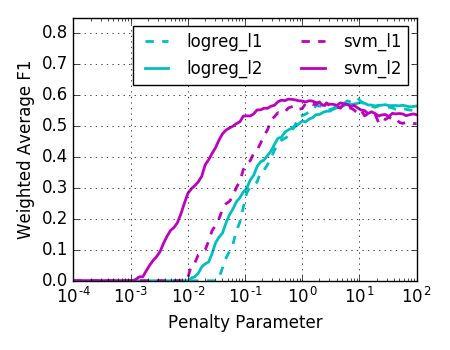
\includegraphics[width=1\linewidth]{reg_K-FOLD}
  \caption{Regularization}
  \label{fig:reg}
\end{minipage}%
\begin{minipage}{.5\linewidth}
  \centering 
  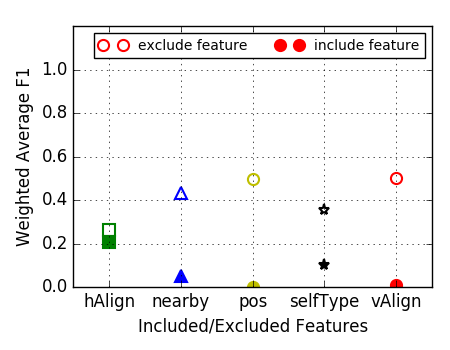
\includegraphics[width=1\linewidth]{incfeatures_K-FOLD_svm_python}
  \caption{Feature Rules Effectiveness}
  \label{fig:fetrule}
\end{minipage}
\end{figure}

\subsection{Feature Selection}

\begin{figure*}[ht]
\centering
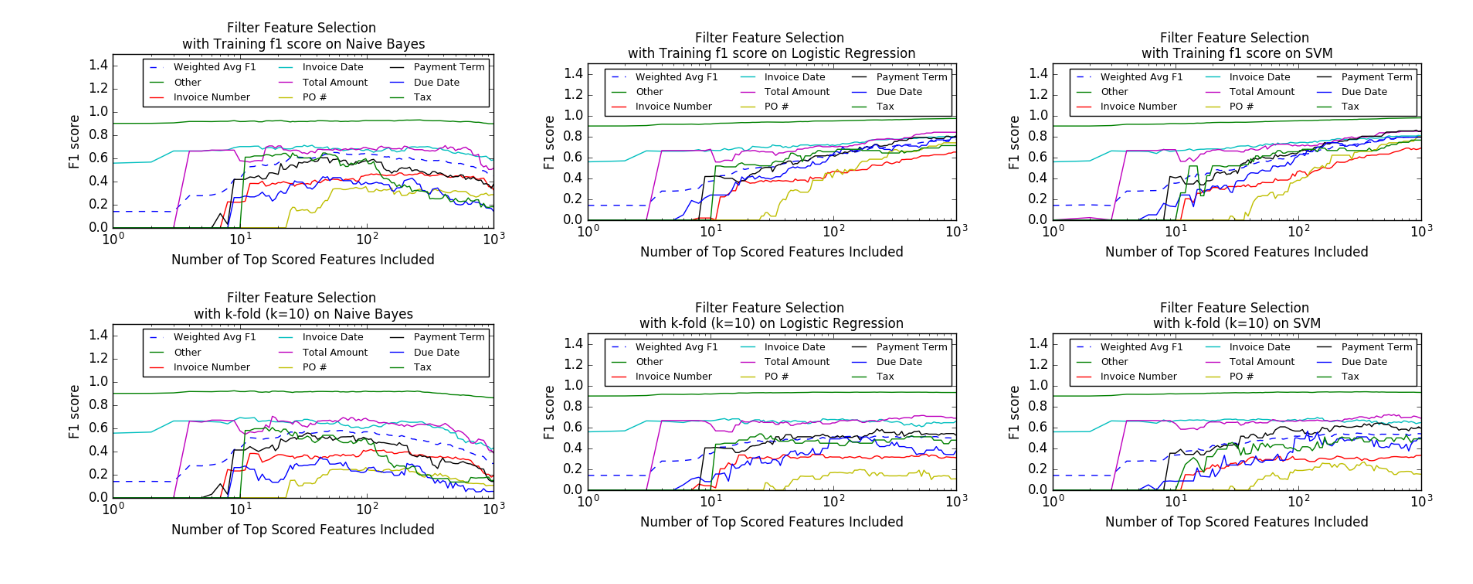
\includegraphics[trim={1cm 0.8cm 0 0}, clip, width=1\linewidth]{filterFS}
\caption{Filter Feature Selection. The solid lines are individual $F_1$ scores for all classes and the dashed line is the weighted average $F_1$ score}
\label{fig:fetsel}
\end{figure*}

%% Feature selection rule effectiveness
Fig.\ref{fig:fetrule} evaluates the effectiveness of each feature selection rule, where solid markers represent weighted average $F_1$ when only that selection rule is included (inclusion set), while hollow markers represent the case when only that rule is excluded (exclusion set). We can easily see that horizontal alignment (hAlign) is the most effective, with best performance in the inclusion set and worst performance in the exclusion set, and is followed by self type (selfTpe), nearby, vertical align (vAlign), and position (pos). It is not a surprise that hAlign is the most effective, as many fields of interests, regardless of the absolute position, are horizontally aligned in a decent number of invoices. On the contrary, while the absolute vertical position was moderately indicative when data size was small, The variety in invoice templates increase dramatically as data set expands, making it harder to derive common properties in layout structure and causing this feature selection rule to be less instructive.

%% Feature selection
Following rule-level analysis, filter feature selection is performed on the individual features to exclude the less indicative ones generated by effective selection rules. First, for every feature, we use the empirical distribution of each feature, $p(x_i)$, and that of each class, $p(y)$, as well as their joint distribution, $p(x_i,y)$, to compute the mutual information MI($x_i, y$) between $x_i$ and $y$, given by the Kullback-Leibler (KL) divergence of the distributions $p(x_i, y)$ and $p(x_i)p(y)$, as
\begin{align*}
\mathrm{MI}(x_i, y) &= \mathrm{KL}(p(x_i, y)\Vert p(x_i)p(y))\\
&=\sum_{x_i\in\{0,1\}}\sum_{y=0}^7p(x_i,y)\log\frac{p(x_i, y)}{p(x_i)p(y)}.
\end{align*}
$\mathrm{MI}(x_i, y)$ thus serves as a score, a large value of which indicates the feature $x_i$ is strongly correlated with the class labels and small otherwise. Therefore, we pick top scored features in our model. To decide how many features 
to include, we sweep the number of top scored features included and use the weighted average $F_1$ score with $k$-fold validation
to threshold desired performance.

Fig.~\ref{fig:fetsel} shows our experimental results for both training $F_1$ score and testing
$F_1$ score computed with $k$-fold cross-validation for three algorithms. For training $F_1$ score,
both SVM and Logistic Regression monotonically increase as more features are included because the
model is overfit. The performance of Naive Bayes, however, first dramatically improves as number of
features increases when feature size is small and then starts to degrade when too many features are
included. This is because Naive Bayes weights probabilities of all features equally and simply
multiply them together. Therefore, the contribution of indicative features to the overall
probability decreases as more features are included, resulting in a downgrade in performance. Similar
but more exaggerated behavior can be observed in testing $F_1$ score for Naive Bayes. Additionally,
Naive Bayes assumes features are independent to each other, which in many cases is not accurate. For
instance, if token 'invoice number' is in nearby region, it is very likely that 'invoice date' and
other header tokens are also in the nearby region. Finally, performance of SVM and Logistic
Regression increases first before reaching constant. The turning point of $F1$ score at 434 number of features is where we threshold amount of features to include, as including more features will 
not improve the performance. 

\subsection{Overall Performance Evaluation}

\begin{table}[!t]
% increase table row spacing, adjust to taste
%\renewcommand{\arraystretch}{1.3}
%if using array.sty, it might be a good idea to tweak the value of
%\extrarowheight as needed to properly center the text within the %cells
\caption{Average Training and Testing Accuracy}
\label{tab:accuracy}
\centering
% Some packages, such as MDW tools, offer better commands for making tables
% than the plain LaTeX2e tabular which is used here.
\begin{tabular}{|c|c|c|}
\hline
 & Training Error (\%) & Testing Error (\%)\\\hline
\begin{tabular}{@{}c@{}}Naive Bayes \\ (9 features)\end{tabular} & 16.17 & 16.43\\\hline
\begin{tabular}{@{}c@{}}Logistic Regression \\ (249 features)\end{tabular} & 10.95 & 14.53\\\hline
\begin{tabular}{@{}c@{}}SVM \\ (157 features)\end{tabular} & 8.81 & 13.99\\\hline
\end{tabular}
\end{table}

\begin{figure*}[ht]
\centering
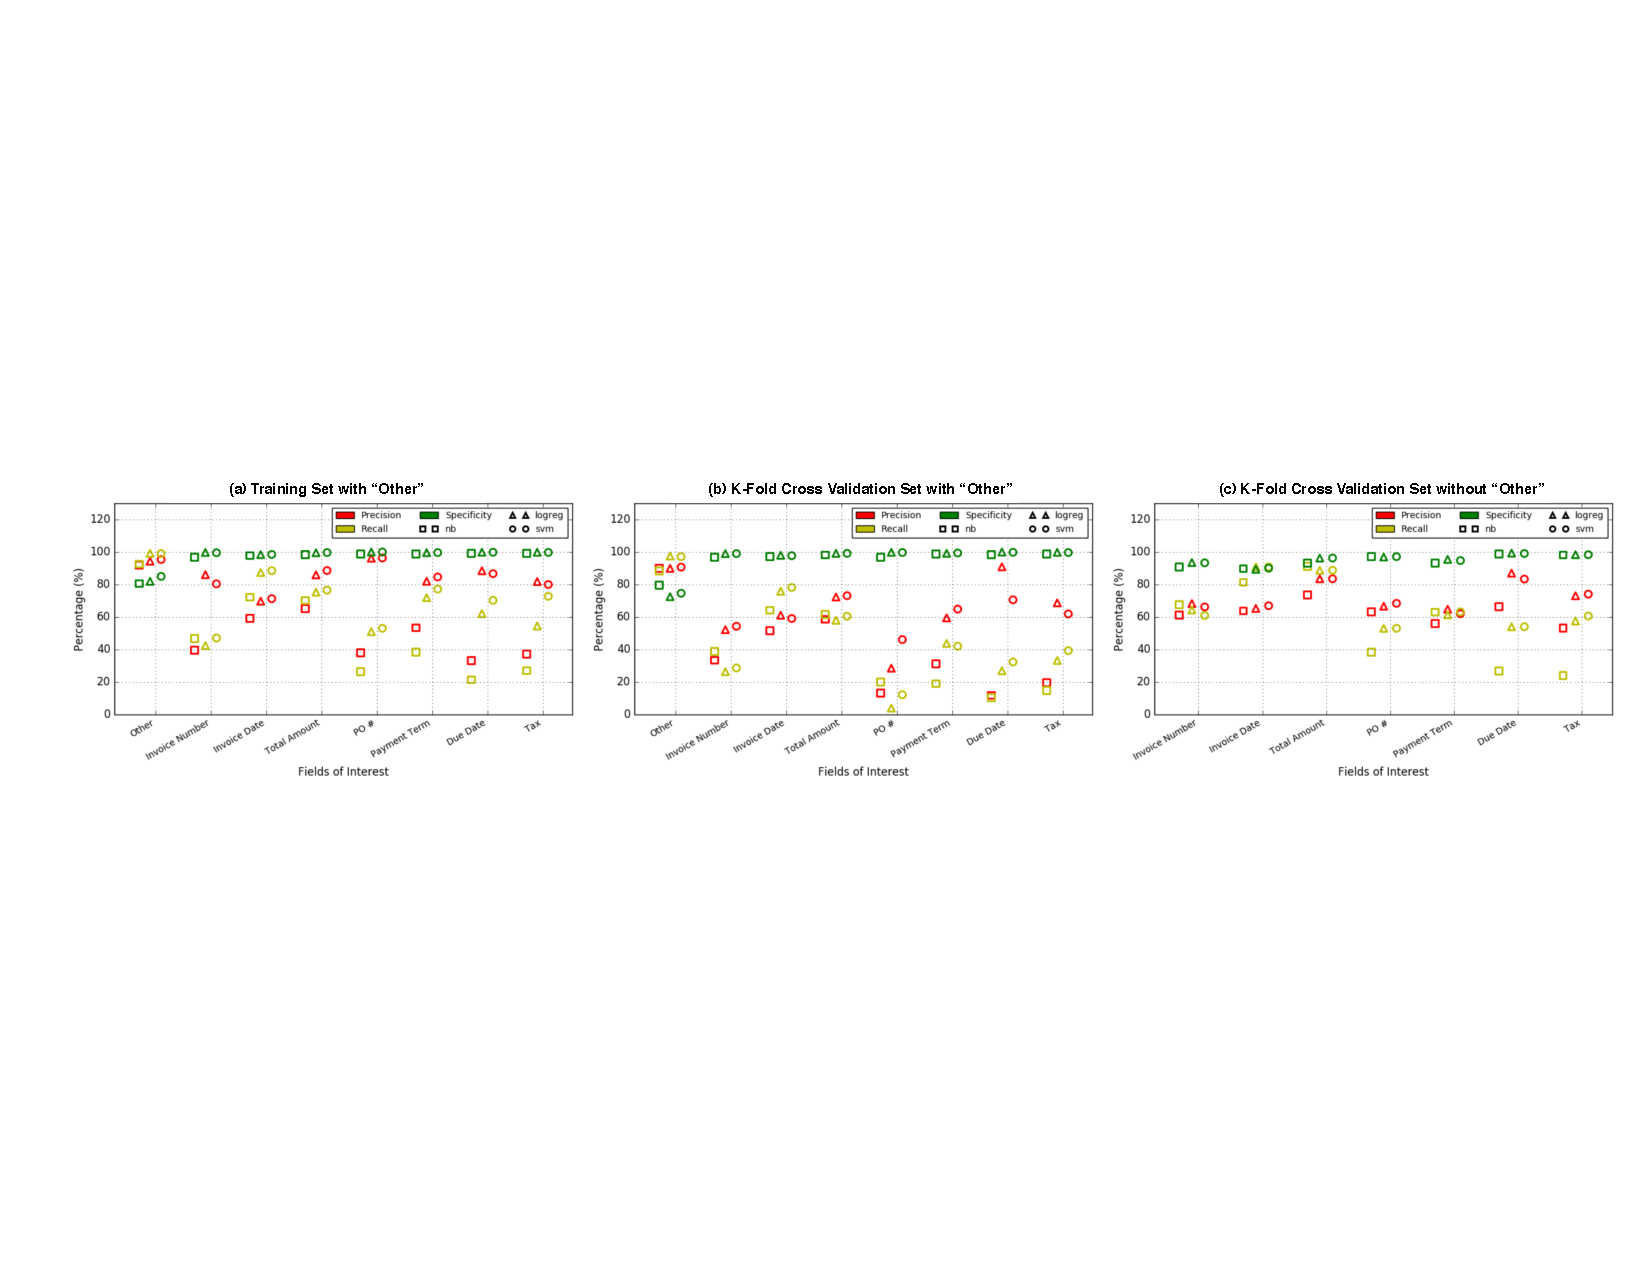
\includegraphics[width=1\linewidth, trim={1cm 8cm 0.3cm 8cm}, clip, ]{model_all.pdf}
\caption{Classifier Overall Performance, measured by Precision, Recall, and Specificity}
\label{fig:model}
\end{figure*}

Table \ref{tab:accuracy} shows the best $k$-fold cross validation accuracy achieved and training accuracy for three algorithms with corresponding number of top scored features.  There is only slight overfitting in Logistic Regression and SVM due to application of regularization and overall accuracy is promising.

Fig. \ref{fig:model} shows the precision, recall, and specificity of all classes and three algorithms on training and test data computed with $k$-fold cross validation. The trade-off between precision and recall can be found in most classes. Fig. \ref{fig:model}(a) shows that our models performs well across all classes on the training data. However, comparison between \ref{fig:model}(a) and (b) shows that our algorithms have a high variance for Invoice Number and PO \#, which suggests overfitting. These fields are especially prone to overfitting because their bag of features vary hugely and we have a especially small quantity of PO \# tokens.

It can be seen from Fig. \ref{fig:model}(a) \& (b) that for almost all classes,  Naive Bayes has a worse performance than Logistic Regression and SVM in terms of both precision and recall.  We believe that this is largely due to the aforementioned fact that the Naive Bayes model makes the assumption that all features are conditionally independent given the class labels, which likely does not hold in this classification context. Logistic Regression and SVM have similar precision in all fields of interest but \textit{PO \#}, \textit{Due Date}, and \textit{Tax}, with SVM performing slightly better. SVM outperforms Logistic Regression for \textit{PO \#}, whereas Logistic Regression has better performance for \textit{Due Date} and \textit{Tax}. One major difference between these fields is that fields that are \textit{PO \#}'s can vary largely in terms of its type and its position in the invoice file, whereas \textit{Due Date} and \textit{Tax} are generally of the same type (date and money, respectively), and can be identified by self type more easily.  This suggests that SVM is better than Logistic Regression at extracting the most useful features among all when making a prediction.

Another important observation is that except \textit{Other} (class label 0), all fields of interest suffer from low recall regardless of which algorithm is used, but have very high specificity, whereas the \textit{Other} field has very high recall but low specificity. This indicates that it is very easy for our learning algorithms to mis-classify fields like \textit{Invoice Number}, \textit{Invoice Date}, etc.\ (class labels 1-7) as \textit{Other},  while there are very few instances where \textit{Other} is classified as the rest of the fields. The reason is that the \textit{Other} field actually contains all different type of fields that are unlabeled in our data, which results in a highly skewed class distribution and leads to a very high tendency for our algorithm to predict a field to be \textit{Other}. This argument can be further corroborated by Fig. \ref{fig:model}(c), which is the same plot but without the \textit{Other} field. It can easily be seen that the performance across all fields of interest dramatically increases, especially for precision and recall. In other words, our algorithm can reliably tell whether a field belongs to one class or another among class labels 1-7, but because of the presence of large amount of tokens belonging to \textit{Other} and \textit{Other} exhibits large range of feature characteristics, our performance suffers from the high rate of misclassifying 1-7 as 0. We believe the issue can be alleviated when more training data are available and more type of fields of interest are labeled in our training data.



%\section{Limitation and Future Work}


\section{Conclusion and Future Work}
Overall, SVM produced the best results because it does not make unnecessary assumptions like Naive Bayes does, and can intelligently find the best margin separating two classes.\\

If we had more time, we would explore more ways to handle overfitting, which includes expanding training data size, and using wrapper model feature selection for more precise results. Further analysis might be worthwhile on the effectiveness of the current set of feature selection rules in capturing the inherent nature of invoice layout, and perform rule-level feature selection on a larger pool of potential feature generation rules. Additionally, current results are largely affected by poor OCR performance, which suggests investigation on more optimized OCR tools or collection of higher quality invoice images.

%\section*{Acknowledgment}

The authors would like to thank... no one


%\pagebreak

\bibliographystyle{ieeetr}
\bibliography{references}

%\appendix 
I love machine learning


%\section{Section Heading Here}
%Section text here.

%\subsection{Subsection Heading Here}
%Subsection text here.

%\subsubsection{Subsubsection Heading Here}
%Subsubsection text here.

% An example of a floating figure using the graphicx package.
% Note that \label must occur AFTER (or within) \caption.
% For figures, \caption should occur after the \includegraphics.
% Note that IEEEtran v1.7 and later has special internal code that
% is designed to preserve the operation of \label within \caption
% even when the captionsoff option is in effect. However, because
% of issues like this, it may be the safest practice to put all your
% \label just after \caption rather than within \caption{}.
%
% Reminder: the "draftcls" or "draftclsnofoot", not "draft", class
% option should be used if it is desired that the figures are to be
% displayed while in draft mode.
%
%\begin{figure}[!t]
%\centering
%\includegraphics[width=2.5in]{myfigure}
% where an .eps filename suffix will be assumed under latex, 
% and a .pdf suffix will be assumed for pdflatex; or what has been declared
% via \DeclareGraphicsExtensions.
%\caption{Simulation results for the network.}
%\label{fig_sim}
%\end{figure}

 %Note that the IEEE typically puts floats only at the top, even when this
 %results in a large percentage of a column being occupied by floats.


% An example of a double column floating figure using two subfigures.
% (The subfig.sty package must be loaded for this to work.)
% The subfigure \label commands are set within each subfloat command,
% and the \label for the overall figure must come after \caption.
% \hfil is used as a separator to get equal spacing.
% Watch out that the combined width of all the subfigures on a 
% line do not exceed the text width or a line break will occur.
%
%\begin{figure*}[!t]
%\centering
%\subfloat[Case I]{\includegraphics[width=2.5in]{box}%
%\label{fig_first_case}}
%\hfil
%\subfloat[Case II]{\includegraphics[width=2.5in]{box}%
%\label{fig_second_case}}
%\caption{Simulation results for the network.}
%\label{fig_sim}
%\end{figure*}
%
% Note that often IEEE papers with subfigures do not employ subfigure
% captions (using the optional argument to \subfloat[]), but instead will
% reference/describe all of them (a), (b), etc., within the main caption.
% Be aware that for subfig.sty to generate the (a), (b), etc., subfigure
% labels, the optional argument to \subfloat must be present. If a
% subcaption is not desired, just leave its contents blank,
% e.g., \subfloat[].


% An example of a floating table. Note that, for IEEE style tables, the
% \caption command should come BEFORE the table and, given that table
% captions serve much like titles, are usually capitalized except for words
% such as a, an, and, as, at, but, by, for, in, nor, of, on, or, the, to
% and up, which are usually not capitalized unless they are the first or
% last word of the caption. Table text will default to \footnotesize as
% the IEEE normally uses this smaller font for tables.
% The \label must come after \caption as always.
%
%\begin{table}[!t]
%% increase table row spacing, adjust to taste
%\renewcommand{\arraystretch}{1.3}
% if using array.sty, it might be a good idea to tweak the value of
% \extrarowheight as needed to properly center the text within the cells
%\caption{An Example of a Table}
%\label{table_example}
%\centering
%% Some packages, such as MDW tools, offer better commands for making tables
%% than the plain LaTeX2e tabular which is used here.
%\begin{tabular}{|c||c|}
%\hline
%One & Two\\
%\hline
%Three & Four\\
%\hline
%\end{tabular}
%\end{table}


% Note that the IEEE does not put floats in the very first column
% - or typically anywhere on the first page for that matter. Also,
% in-text middle ("here") positioning is typically not used, but it
% is allowed and encouraged for Computer Society conferences (but
% not Computer Society journals). Most IEEE journals/conferences use
% top floats exclusively. 
% Note that, LaTeX2e, unlike IEEE journals/conferences, places
% footnotes above bottom floats. This can be corrected via the
% \fnbelowfloat command of the stfloats package.


% use section* for acknowledgment

% trigger a \newpage just before the given reference
% number - used to balance the columns on the last page
% adjust value as needed - may need to be readjusted if
% the document is modified later
%\IEEEtriggeratref{8}
% The "triggered" command can be changed if desired:
%\IEEEtriggercmd{\enlargethispage{-5in}}

% references section

% can use a bibliography generated by BibTeX as a .bbl file
% BibTeX documentation can be easily obtained at:
% http://mirror.ctan.org/biblio/bibtex/contrib/doc/
% The IEEEtran BibTeX style support page is at:
% http://www.michaelshell.org/tex/ieeetran/bibtex/
%\bibliographystyle{IEEEtran}
% argument is your BibTeX string definitions and bibliography database(s)
%\bibliography{IEEEabrv,../bib/paper}
%
% <OR> manually copy in the resultant .bbl file
% set second argument of \begin to the number of references
% (used to reserve space for the reference number labels box)
%\begin{thebibliography}{1}

%\bibitem{IEEEhowto:kopka}
%H.~Kopka and P.~W. Daly, \emph{A Guide to \LaTeX}, 3rd~ed.\hskip 1em plus
  %0.5em minus 0.4em\relax Harlow, England: Addison-Wesley, 1999.

%\end{thebibliography}

\end{document}


